\section{Estimation of mutual information and missing mass problem}
\label{sec:missing_mass}
%
%
%
In this section, we discuss how to estimate the mutual information from a finite
sample, which may not cover the full distribution. To control the estimation
error, we first introduce the concept of \emph{missing mass}.
%
\subsection{The missing mass problem}
\label{sec:missing-mass}
%
%
Let $\cX$ be a countable set and suppose that $\Sample_1, \ldots, \Sample_k \sim \mu \in \cM_1(\cX^n)$ independently.
In the following $x$ is used as an element of $\cX^n$ rather than the query (as in \Cref{sec:epistemic}).
Then, the missing mass is defined as the random variable
\begin{align*}
  U_k = \sum_{\sample \in \cX^n} \mu(\sample) \, \xi(\sample)~,
  \qquad
  \xi(\sample) = \mathbb{I}\{\sample \not \in \{\Sample_1, \ldots, \Sample_k\}\}~.
\end{align*}
%
Here we are primarily interested in two questions: \emph{(i)} how quickly $U_k$ approaches the expected missing mass $\E U_k$, where it is not hard to see that
\begin{align*}
  \E U_k = \sum_{\sample \in \cX^n} \mu(\sample) (1-\mu(\sample))^k~;
\end{align*}
and \emph{(ii)} we are also interested in giving an estimate for $\E U_k$ given $\mu$ and $k$.
%
The first question is answered by the following theorem:
%
\begin{theorem}[Concentration of a missing mass~\citep{berend2013concentration}]
  \label{thm:missing-mass-concentration}
  For any $t > 0$, we have an upper-tail bound
  \begin{align*}
    \P\pr{U_k > \E U_k + t} \leq e^{-t k^2}~,
  \end{align*}
  and moreover for a universal constant $c \approx 7.6821$, we have an lower-tail bound
  \begin{align*}
    \P\pr{U_k < \E U_k - t} \leq e^{-c t k^2}~.
  \end{align*}
\end{theorem}
Notably $U_k$ exhibits a sub-gaussian concentration (i.e. $1/\sqrt{k}$), which is surprisingly fast.
As we will see next, the main bulk of the error incurred for missing a subset of the support is hidden in $\E U_k$.

In particular, when $\cX$ is finite with $|\cX|=N$, \citet{berend2012missing} showed that
\[
  \E U_k \leq
  \begin{cases}
    e^{-\frac{n}{N}}, & \text{ if } n \leq N;\\
    \frac{N}{e \, n}, & \text{ if } n > N.
  \end{cases}
\]

In the countably infinite $\cX$, we cannot generally have a non-trivial bound on $\E U_k$ only in terms of $n$.
In fact, \citet{berend2012missing} show a bound that depends on $\mu$ which is expected to be finite for  rapidly decaying atoms.
Interestingly, when the entropy of $\mu$ is bounded, one has the following result \citep{berend2017expected}:
\begin{theorem}
  \label{thm:missing-mass-countable}
  Let $H(\mu) \leq h < \infty$.
  For all $n \geq 1$, we have $\E U_k \leq \frac{h}{\sum_{i=1}^k i^{-1}} \leq \frac{h}{\ln(n)}.$
\end{theorem}
%
Note that these estimates are very pessimistic, and in reality we expect the expected missing mass to be significantly smaller.
%
Since natural (and many artificial) languages follow a Zipf distribution~\citep{piantadosi2014zipf}, we expect that $\E[U_k]$ should be much smaller than in the above cases, since sampling from the tail of a Zipf distribution is a rare event.
%
In \Cref{sec:zipf} we show the following:
\begin{corollary}[Expected missing mass of Zipf distribution]
  Consider distribution $\mu(i) = i^{-\alpha} / H(\alpha, N)$ for $i \in [N]$, where $\alpha > 1$ and $H(\alpha, N) = \sum_{i=1}^N i^{-\alpha}$.
  Then, for any $\beta > 0$,
  \begin{align*}
    \E[U_k] = \mathcal{O}\Big(k^{-(\frac{\alpha-1}{\alpha} - \beta)} \Big)~.
  \end{align*}
\end{corollary}
\begin{proof}
  The statement followss by combining \Cref{lem:missing-mass-accrual-bounds,prop:zipf}.
\end{proof}
%
%
\subsection{Estimating mutual information from the partial support}
%
Our goal is to estimate
\begin{align*}
  I (\mu) =
  D_{\KL}(\mu, \mu^{\otimes}) = \sum_{\sample \in \cX^n} \mu(\sample) \ln\pr{\frac{\mu(x)}{\mu^{\otimes}(\sample)}}
\end{align*}
%
by only having access to $\Sample_1, \ldots, \Sample_k \sim \mu$.
Note that that the sample might cover only some part of the support of $\cX$ and therefore we are facing a missing mass problem.
In the following we consider estimator $\widehat I_k(\gamma)$ given by \Cref{alg:MI}.
%
%


%
In particular in \Cref{sec:proof-of-emp-wav-MI} we show the following
%
%
\begin{theorem}
  \label{thm:emp-wav-MI}
  Fix $\tilde \cX \subseteq \cX^n$.
  Fix $\gamma_1 > 0$ and suppose that $\gamma_2 \geq n (1-Z) + \gamma_1$.
  Then for any fixed $\delta \in (0,1)$, with probability at least $1-\delta$,
  \begin{align*}
    (1 - \ve_k) \, \widehat I_k(\gamma_1, \gamma_2)
    -
    \pr{
    |\tilde \cX|\gamma_1
    +
    \ln \pr{ e + \frac{e}{\gamma_1}} \pr{ \mu(\cX^n \setminus \tilde{\cX}) + \ve_k }
    }
    \leq
    I(\mu)
  \end{align*}
  where
  \begin{align*}
    \ve_k = \E U_k + \sqrt{\frac{\ln(\frac{1}{\delta})}{k}}~.
  \end{align*}
\end{theorem}
%
In particular, \Cref{thm:emp-wav-MI} implies the following:
%
\begin{corollary}
  \label{cor:MI-1}
  Under conditions of \Cref{thm:emp-wav-MI}, there exists $(\gamma^*_1, \gamma^*_2) \in (0, 1)^2$ such that
  \begin{align*}
    (1 - \ve_k) \, \widehat I_k(\gamma^*_1, \gamma_2^*)
    -
    \pr{
    \frac{1}{k}
    +
    (1+
    n \, \ln \big( 1 + k \, |\cX|) \big) \, \ve_k
    }
    \leq
    I(\mu)~.
  \end{align*}
\end{corollary}
%

%
Note that, choosing any of the upper bounds on $\E U_k$ discussed in \Cref{sec:missing-mass}, we can see that \Cref{cor:MI-1} implies asymptotic convergence in as a sense
\begin{align*}
  \lim_{k \to \infty} \widehat I_k(\gamma^*_1, \gamma_2^*) \leq I(\mu)~.
\end{align*}

\subsection{Proof of \Cref{thm:emp-wav-MI}}
\label{sec:proof-of-emp-wav-MI}
%
The proof will heavily rely on the simple fact that
\begin{align}
  \label{eq:PX-i-xi}
 1-\xi(\sample) \,
 = \begin{cases}
 1, & \text{ if $\sample \in \{\Sample_1,\ldots,\Sample_k\}$;} \\
 0, & \text{ otherwise.}
 \end{cases}
\end{align}
%
Recalling that $S = \big\{i \in [k] ~:~ \Sample_i \neq \Sample_j \quad \forall j < i \big\}$, this immediately implies the following connection between $U_k$ and the quantities used in \Cref{alg:MI}:
\begin{proposition}
  \label{prop:wav-missing-mass}
  We have that
  \begin{align*}
    \sum_{j \in S} \mu(\Sample_j)
    =
    \sum_{\sample \in \cX^n} (1-\xi(\sample)) \, \mu(\sample)
    = 1 - U_k~.
    \end{align*}
\end{proposition}
%
Recall that the product distribution of $\mu$ is defined as
\begin{align*}
  \mu^{\otimes}(\sample)
  = \prod_{i=1}^n \sum_{\sample^{\backslash i}} \mu(\sample_1, \ldots, \sample_{i-1}, \sample_i, \sample_{i+1}, \ldots, \sample_n)~.
\end{align*}
Note that we use $\sum_{\sample^{\backslash i}} \mu(\cdots)$ instead of $\mu(\sample_i)$ since these are not necessarily equal for some $\mu$.
%
% Introducing a one-dimensional version of $\xi$, 
% for $i \in [n]$ and $z \in \cX$, as
% \begin{align*}
%   \xi_i(z) = \mathbb{I}\{z \not \in \{\Sample_{1,i}, \ldots, \Sample_{k,i}\}\}~,
% \end{align*}
% we introduce the normalization factors
% \begin{align*}
%   \Normfactor = \sum_{\sample \in \cX^n} (1-\xi(\sample)) \mu(\sample)~, \qquad
%   \Normfactor^{\otimes} = \prod_{i=1}^n \sum_{z \in \cX} (1-\xi_i(z)) \sum_{\sample^{\backslash i}} \mu(\sample_1, \ldots, \sample_{i-1}, z, \sample_{i+1}, \ldots, \sample_n)~.
% \end{align*}
%
% We first note that by the definition of $\widehat \mu^{\otimes}$, for any $\sample' \in \cX^n$,
% %
% \begin{align*}
%   \widehat \mu^{\otimes}(\sample')
%   &=
%     \prod_{i=1}^n
%     \frac{\sum_{\sample^{\backslash i}} \mu(\sample_1, \ldots, \sample_{i-1}, \sample_i', \sample_{i+1}, \ldots, \sample_n)}{
%     \sum_{j \in S} \sum_{\sample^{\backslash i}} \mu(\sample_1, \ldots, \sample_{i-1}, \Sample_{j,i}, \sample_{i+1}, \ldots, \sample_n)
%     }\\
%   &=
%     \prod_{i=1}^n
%     \frac{\sum_{\sample^{\backslash i}} \mu(\sample_1, \ldots, \sample_{i-1}, \sample_i', \sample_{i+1}, \ldots, \sample_n)}{
%     \sum_{z \in \cX} (1-\xi_i(z)) \sum_{\sample^{\backslash i}} \mu(\sample_1, \ldots, \sample_{i-1}, z, \sample_{i+1}, \ldots, \sample_n)
%     }\\
%   &=
%     \frac{\mu^{\otimes}(\sample')}{\Normfactor^{\otimes}}~,
% \end{align*}
% where the second equality comes from the definition of $\xi_i$ and the fact that the $X_i$ are all different.
%
%
Now, using the definitions of $ \widehat I_k$, $\widehat \mu$, and $\widehat \mu^{\otimes}$,
\begin{align*}
  \widehat I_k(\gamma_1, \gamma_2)
  % &=
  %   \frac{1}{Z} \sum_{i \in S} \mu(\Sample_i) \pr{ \ln\pr{\frac{\mu(\Sample_i)}{Z} + \frac{\gamma_1}{Z}
  %   }
  %   - \ln \pr{\widehat \mu^{\otimes}(\Sample_i) + \frac{\gamma_2}{Z}}
  %   }\\
  &=
    \frac{1}{\Normfactor} \sum_{i \in S} \mu(\Sample_i) \pr{ \ln\pr{\frac{\mu(\Sample_i)}{\Normfactor} + \gamma_1
    }
    - \ln \pr{\widehat \mu^{\otimes}(\Sample_i) + \gamma_2}
    } \\
  &=
    \frac{1}{\Normfactor} \sum_{\sample \in \cX^n} (1-\xi(\sample)) \, \mu(\sample) \pr{ \ln\pr{\frac{\mu(\sample)}{\Normfactor} + \gamma_1
    }
    - \ln \pr{\widehat \mu^{\otimes}(\Sample_i) + \gamma_2}
    } \tag{by \cref{eq:PX-i-xi} }\\
  &=
    \frac{1}{\Normfactor} \sum_{\sample \in \cX^n} (1-\xi(\sample)) \, \mu(\sample) \pr{ \ln\pr{\frac{\mu(\sample) + \gamma_1}{\mu^{\otimes}(\sample) + \gamma_1}
    }
    + \ln\pr{\frac{\mu^{\otimes}(\sample) + \gamma_1}{\widehat \mu^{\otimes}(\sample) + \gamma_2}}
    + \ln\frac{1}{\Normfactor}
    }\\
  % &\le
  %   \frac{1}{\Normfactor} \sum_{\sample \in \cX^n} (1-\xi(\sample)) \, \mu(\sample) \pr{ \ln\pr{\frac{\mu(\sample) + \gamma}{\mu^{\otimes}(\sample) + \gamma}}
  %   }
  %   +
  %   \ln \frac{\Normfactor^{\otimes}}{\Normfactor}\\
    &=
      \underbrace{
      \frac{1}{\Normfactor}\sum_{\sample \in \cX^n} \mu(\sample) \ln \pr{ \frac{\mu(\sample) + \gamma_1}{\mu^{\otimes}(\sample) + \gamma_1}}
      }_{(i)}
      +
      \underbrace{
      \frac{1}{\Normfactor} \sum_{\sample \in \cX^n} \xi(\sample) \, \mu(\sample) \ln \pr{ \frac{\mu^{\otimes}(\sample) + \gamma_1}{\mu(\sample) + \gamma_1}}
      }_{(ii)}
      +
      \underbrace{
      \ln \frac{1}{\Normfactor}
      }_{(iii)}\\
      &+
        \underbrace{
        \frac{1}{\Normfactor} \sum_{\sample \in \cX^n} (1-\xi(\sample)) \, \mu(\sample)
      \ln\pr{\frac{\mu^{\otimes}(\sample) + \gamma_1}{\widehat \mu^{\otimes}(\sample) + \gamma_2}}
      }_{(iv)}
\end{align*}
%
Now we control each of the terms individually.
%
To control $(i)$ we will first need the fact that $q \ln((q+\gamma_1)/p) \leq q \ln(q/p) + \gamma_1$ for any $q,p \in [0,1], \gamma_1 > 0$.
Note that this follows since
\begin{align}
  \label{eq:MI-1}
  q \ln\pr{\frac{q+\gamma_1}{p}}
  = q \ln\pr{1+\frac{\gamma_1}{q}} + q \ln\pr{\frac{q}{p}}
  \le \gamma_1 + q \ln\pr{\frac{q}{p}}
\end{align}
using that $\ln(1+a) \le a$ for $a > -1$.
Getting back to $(i)$, and using the aforementioned inequality, we get
\begin{align*}
  (i) &= \frac{1}{\Normfactor}\sum_{\sample \in \cX^n} \mu(\sample) \ln \pr{ \frac{\mu(\sample) + \gamma_1}{\mu^{\otimes}(\sample) + \gamma_1}}\\
      &= \frac{1}{\Normfactor}\sum_{\sample \in \tilde{\cX}} \mu(\sample) \ln \pr{ \frac{\mu(\sample) + \gamma_1}{\mu^{\otimes}(\sample) + \gamma_1}}
        + \frac{1}{\Normfactor}\sum_{\sample \in \cX^n \setminus \tilde{\cX}} \mu(\sample) \ln \pr{ \frac{\mu(\sample) + \gamma_1}{\mu^{\otimes}(\sample) + \gamma_1}}\\
      &\leq \frac{1}{\Normfactor}\sum_{\sample \in \tilde{\cX}} \mu(\sample) \ln \pr{ \frac{\mu(\sample) + \gamma_1}{\mu^{\otimes}(\sample) + \gamma_1}}
        + \frac{1}{\Normfactor} \, \ln \pr{ \frac{1 + \gamma_1}{\gamma_1}} \, \mu(\cX^n \setminus \tilde{\cX}) \\
  &\le
    \frac{1}{\Normfactor} \sum_{\sample \in \tilde \cX} \pr{ \mu(\sample) \ln \pr{ \frac{\mu(\sample)}{\mu^{\otimes}(\sample)}} + \gamma_1 }
    +
    \frac{1}{\Normfactor} \, \ln \pr{1+\frac{1}{\gamma_1}} \, \mu(\cX^n \setminus \tilde{\cX})
    \tag{by \Cref{eq:MI-1}}\\
&= \frac{1}{\Normfactor}\left(D_{\KL}(\mu, \mu^{\otimes}) + |\tilde \cX| \, \gamma_1\right)
        +
    \frac{1}{\Normfactor} \, \ln \pr{1+\frac{1}{\gamma_1}} \, \mu(\cX^n \setminus \tilde{\cX})~.
\end{align*}
%
Furthermore,
\begin{align*}
  (ii)
  \leq
  \frac{1}{\Normfactor} \, \sum_{\sample \in \cX^n} \xi(\sample) \, \mu(\sample) \ln \pr{1 + \frac{1}{\gamma_1}}
  =
  \frac{1-\Normfactor}{\Normfactor} \, \ln \pr{1 + \frac{1}{\gamma_1}}~.
\end{align*}
%
Next, observe that $(iii) \leq \ln(1/\Normfactor)$.
Finally, term $(iv)$ is controlled through the following fact shown at the end of this section:
\begin{lemma}
  \label{lem:controlling-product-mu-gap}
  Suppose that $\gamma_1 \geq 0$ while $\gamma_2 \geq \gamma_1 + n (1-Z)$.
  Then,
  \begin{align*}
    \frac{1}{\Normfactor}\sum_{\sample \in \cX^n} (1-\xi(x)) \mu(\sample) \ln \pr{ \frac{\mu^{\otimes}(\sample) + \gamma_1}{\widehat \mu^{\otimes}(\sample) + \gamma_2}}
    \leq 0~.
  \end{align*}
\end{lemma}
%
%
Putting everything together, we obtain
\begin{align*}
  \widehat I_k(\gamma_1, \gamma_2)
  &\leq
  \frac{1}{\Normfactor}\left(D_{\KL}(\mu, \mu^{\otimes}) + |\tilde \cX|\gamma_1\right)
  +
  \frac{1}{\Normfactor} \, \ln \pr{ 1 + \frac{1}{\gamma_1}} \pr{ \mu(\cX^n \setminus \tilde{\cX}) + 1-\Normfactor }
  +
  \ln(1/\Normfactor)~.
\end{align*}
%
Finally, multiplying through by $\Normfactor$ the entire inequality, and using the fact that $\Normfactor \ln(1/\Normfactor) \leq 1-\Normfactor$, we get
\begin{align*}
  \Normfactor \, \widehat I_k(\gamma_1, \gamma_2)
  &\leq
  D_{\KL}(\mu, \mu^{\otimes}) + |\tilde \cX|\gamma_1
  +
  \ln \pr{ 1 + \frac{1}{\gamma_1}} \pr{ \mu(\cX^n \setminus \tilde{\cX}) + 1-\Normfactor }
  +
    1 - \Normfactor\\
  &\leq
    D_{\KL}(\mu, \mu^{\otimes}) + |\tilde \cX|\gamma_1
  +
  \ln \pr{ e + \frac{e}{\gamma_1}} \pr{ \mu(\cX^n \setminus \tilde{\cX}) + 1-\Normfactor }.
\end{align*}
%
%
%
To complete the proof we need to give a lower bound on $\Normfactor$.
Note that $\Normfactor = 1 - U_k$ by the definition of $\Normfactor$ and \Cref{prop:wav-missing-mass}, and so by \Cref{thm:missing-mass-concentration}
\begin{align*}
  \P\pr{1 - \E U_k > 1 - U_k + t} \leq e^{-t k ^2}~.
\end{align*}
Using this concentration bound together with the choices of $\gamma$ (also setting $\delta_{\supp}=0$ for the first inequality in the main statement) completes the proof of \Cref{thm:emp-wav-MI}.
\QED

\begin{proof}[Proof of \Cref{lem:controlling-product-mu-gap}]
Observe that
\begin{align*}
  \widehat \mu^{\otimes}(\sample)
  &=
    (1-\xi(\sample)) \, \prod_{j=1}^n \sum_{t \in S : X_{t,j} = x_j} \hat \mu(X_{t,1}, \ldots, x_j, \ldots, X_{t,n})\\
  &=
    \frac{1}{Z^n} \, (1-\xi(\sample)) \, \prod_{j=1}^n \sum_{t \in S : X_{t,j} = x_j} \mu(X_{t,1}, \ldots, x_j, \ldots, X_{t,n})\\
  &=
    \frac{1}{Z^n} \, (1-\xi(\sample)) \, \prod_{j=1}^n \sum_{x' \in \cX^n} (1-\xi(x')) \, \mathbb{I}\{x'_j = x_j\} \, \mu(x_1', \ldots, x_j, \ldots, x_n')\\
  &=
    \frac{1}{Z^n} \, (1-\xi(\sample)) \, \prod_{j=1}^n \sum_{{x'}^{\delj}} (1-\xi(x'_1, \ldots, x_j, \ldots, x'_n)) \, \mu(x_1', \ldots, x_j, \ldots, x_n')~.
\end{align*}
% 
Now, using that fact that
\begin{align*}
  &\sum_{{x'}^{\delj}} \xi(x'_1, \ldots, x_j, \ldots, x'_n) \, \mu(x_1', \ldots, x_j, \ldots, x_n')\\
  &\qquad\leq
    \sum_{{x'}^{\delj}, x_j} \xi(x'_1, \ldots, x_j, \ldots, x'_n) \, \mu(x_1', \ldots, x_j, \ldots, x_n')\\
  &\qquad= 1-Z
\end{align*}
    %
we arrive at
%
\begin{align*}
  \widehat \mu^{\otimes}(\sample)
  &\geq
    \frac{1}{Z^n} \, (1-\xi(\sample)) \, \pr{ \prod_{j=1}^n \pr{ \sum_{{x'}^{\delj}} \mu(x_1', \ldots, x_j, \ldots, x_n')
    + Z - 1
    }}_+\\
  &\stackrel{(a)}{\geq}
    \frac{1}{Z^n} \, (1-\xi(\sample)) \, \pr{ \prod_{j=1}^n \sum_{{x'}^{\delj}}  \mu(x_1', \ldots, x_j, \ldots, x_n')
    - n (1-Z) }_+\\
  &=
    \frac{1}{Z^n} \, (1-\xi(\sample)) \pr{ \mu^{\otimes}(x) - n \, (1-Z) }_+
  % &\geq
  %   \frac{1}{Z^n} \, (1-\xi(\sample)) \, \mu^{\otimes}(x)
  %   + \frac{(1 - Z)^n}{Z^n} \, (1-\xi(\sample))
\end{align*}
where to get $(a)$ we used:
%
\begin{proposition}
  For any $p_1, \ldots, p_n \in [0,1]$ and $a \geq 0$, we have
  \begin{align*}
    \prod_{i=1}^n (p_i - a) \geq \big( \prod_{i=1}^n p_i \big) - n \, a~.
  \end{align*}
\end{proposition}
\begin{proof}
  The statement following by lower-bounding the left-hand side by its linearization in $a$ (derivative at $0$), while realizing that it is a convex function of $a$.
\end{proof}
% 
The above gives us that
%
\begin{align*}
  &\frac{1}{\Normfactor}\sum_{\sample \in \cX^n} (1-\xi(x)) \mu(\sample) \ln \pr{ \frac{\mu^{\otimes}(\sample) + \gamma_1}{\widehat \mu^{\otimes}(\sample) + \gamma_2}}\\
  &\qquad\leq
    \frac{1}{\Normfactor}\sum_{\sample \in \cX^n} (1-\xi(x)) \mu(\sample) \ln \pr{ \frac{\mu^{\otimes}(\sample) + \gamma_1}{\frac{1}{Z^n} \, (1-\xi(\sample)) \pr{ \mu^{\otimes}(x) - n (1 - Z)}_+ + \gamma_2}}
\end{align*}
%
and focusing on the case $1 - \xi(x) = 1$ (otherwise both sides are $0$) the above equals to
\begin{align*}
  &\frac{1}{\Normfactor}\sum_{\sample \in \cX^n} \mu(\sample) \ln \pr{ \frac{\mu^{\otimes}(\sample) + \gamma_1}{\frac{1}{Z^n} \, \pr{ \mu^{\otimes}(x) - n (1 - Z)}_+ + \gamma_2}}\\
  &\leq
    \frac{1}{\Normfactor}\sum_{\sample \in \cX^n} \mu(\sample) \ln \pr{ \frac{\mu^{\otimes}(\sample) + \gamma_1}{(\mu^{\otimes}(x) - n (1 - Z))_+ + \gamma_2}}\\
  &\leq
    \frac{1}{\Normfactor}\sum_{\sample \in \cX^n} \mu(\sample) \ln \pr{ \frac{\mu^{\otimes}(\sample) + \gamma_1}{\mu^{\otimes}(x) - n (1 - Z) + \gamma_2}}\\
  &\leq 0
\end{align*}
by setting $\gamma_2 \geq \gamma_1 + n (1-Z)$.
\end{proof}

\subsection{Expected missing mass under Zipf distribution}
\label{sec:zipf}
%
We will rely on some machinery used by \cite{ohannessian2010distribution} who
established distribution-dependent bounds on the expected missing mass.
%
As before let $\mu$ be supported on a countable set.
The \emph{accrual function} is defined as
\begin{align*}
  F(v) = \sum_{\mu(i) \leq v} \mu(i) \qquad (v \in [0,1])
\end{align*}
and moreover the \emph{accrual rates} are defined as
\begin{align*}
  \underline{\rho} = \liminf_{v \to 0} \frac{\ln F(v)}{\ln v}~, \qquad
  \overline{\rho} = \limsup_{v \to 0} \frac{\ln F(v)}{\ln v}
\end{align*}

We use the following result:
\begin{lemma}[{\citealp[Theorem~1]{ohannessian2010distribution}}]
  \label{lem:missing-mass-accrual-bounds}
  Let \(\mu\) have lower and upper accrual rates \(0 < \underline{\rho} \leq \overline{\rho} < \infty\). Then for every \(\beta > 0\) there exists \(k_0\) such that for all \(k > k_0\) we have:
  \begin{align*}
    k^{-(\overline{p}+\beta)} \leq \mathbb{E}[U_k] \leq k^{-(\underline{p}-\beta)}
  \end{align*}
or, equivalently, for every \(\beta > 0\) we have that \(\mathbb{E}[U_k]\) is both \(\Omega(k^{-(\overline{p}+\beta)})\) and \(\mathcal{O}(k^{-(\underline{p}-\beta)})\).

\end{lemma}
%
\begin{proposition}
  \label{prop:zipf}
  Consider the distribution $\mu(v) = i^{-\alpha} / H(\alpha, N)$ for $i \in [N]$ where $\alpha > 1$ and $H(\alpha, N) = \sum_{i=1}^N i^{-\alpha}$.
  Then, $\underline{\rho} = \Omega(\frac{\alpha-1}{\alpha})$ as $N \to \infty$.
\end{proposition}
\begin{proof}
  The idea is to use \Cref{lem:missing-mass-accrual-bounds} to give an upper bound on
  the missing mass. Therefore, we need to establish a lower bound on $\ln F(v)$.
  For now, abbreviate
  \begin{align*}
    u = (v \, H(\alpha, N))^{-\frac{1}{\alpha}}~.
  \end{align*}

  First note that for some $1 \leq u \leq N$
  \begin{align*}
    \sum_{i \geq u}^N i^{-\alpha} \geq \int_{u}^N (1+i)^{-\alpha} \diff i
    =
    \frac{1}{\alpha - 1} \, \pr{ (1+u)^{1-\alpha} - (1 + N)^{1-\alpha} }~.
  \end{align*}
%
  On the other hand,
  %
  \begin{align*}
    \sum_{i=1}^N i^{-\alpha} \leq \int_{1}^N (1+i)^{-\alpha} \diff i
    \leq
    \frac{1}{\alpha - 1} \, ( 1 - N^{1-\alpha} )~.
  \end{align*}
%
  So,
  \begin{align*}
    \ln F(v)
    &\geq
    \ln\pr{
    (1 + u)^{1-\alpha} - (1 + N)^{1-\alpha}
    }
      - \ln(1 - N^{1-\alpha})\\
    &\geq
    \ln\pr{
      (1 + u)^{1-\alpha} - (1 + N)^{1-\alpha}
    }
  \end{align*}
and then
  \begin{align*}
    \ln F(v)
    &= \Omega\pr{(1-\alpha) \ln(1 + u)} \qquad (\text{as} \, N \to \infty)\\
    &= \Omega\pr{(1-\alpha) \ln(u)} \\
    &= \Omega\pr{(1-\alpha) \ln((v \, H(\alpha, N))^{-\frac{1}{\alpha}})} \\
    &= \Omega\pr{\frac{\alpha-1}{\alpha} \, \ln(v) + \frac{\alpha-1}{\alpha} \ln H(\alpha, N)} \\
    &= \Omega\pr{\frac{\alpha-1}{\alpha} \, \ln(v)}~.
  \end{align*}
%
\end{proof}

\paragraph{Data-dependent estimate of the expected missing mass}
\label{sec:missing-mass-data-dependent}
%
We perform an experiment designed to give a data-dependent estimate of the expected missing mass $\E[U_k]$ for some specific datasets.
Clearly, we cannot simply apply a concentration bound discussed in \Cref{sec:missing-mass} since the complete support of the pseudo joint distribution derived from the LLM is unknown.
To this end, we approximate it with a finite support driven by the language model itself.
In particular, given a query we sample responses (at temperature $0.9$) until their total probability mass reaches $0.95$ or we reach $1000$ responses per query.
In case of TriviaQA, we performed $1233$ queries in total.
The mean and the median number of unique responses per query was eventually $118.3$ and $22$, respectively.
In case of the AmbigQA dataset, we performed $700$ queries, while the mean and the median number of unique responses
was $277$ and $69$, respectively.
%In both cases we sampled $k=1000$, responses to each query with temperature $0.9$.

At this point, we denote the set of responses by $\tilde \cX$ and let $\tilde U_k$ be the missing mass computed on $\tilde \cX$.
Then, we have
\begin{align*}
  \E[U_k] \leq U_k + \sqrt{\frac{\ln(\frac{1}{\delta})}{k}}
  \leq \tilde U_k + U_k - \tilde U_k + \sqrt{\frac{\ln(\frac{1}{\delta})}{k}}
  \leq \tilde U_k + 1 - P(\tilde\cX) + \sqrt{\frac{\ln(\frac{1}{\delta})}{k}}~,
\end{align*}
which can be computed in practice.
%
In \Cref{fig:missing-mass} we present our results in the form of empirical distributions of different quantities, where each observation corresponds to a single query.
%
%
    %
We compute the bounds for TriviaQA and AmbigQA datasets (see \Cref{sec:experiments} for details about these datasets).
%
From \Cref{fig:missing-mass} we can conclude that the expected missing mass for both datasets is very small: Both the missing mass computed on $\tilde{\cX}$ and the resulting upper bound on $\E[U_k]$ 
are concentrated close to $0$, while the cumulative probability of the approximate support $\tilde{\cX}$ is close to $1$ most of the time, showing that our approximations are meaningful.
\begin{figure}[H]
  \centering
  \begin{subfigure}[b]{0.48\linewidth}
    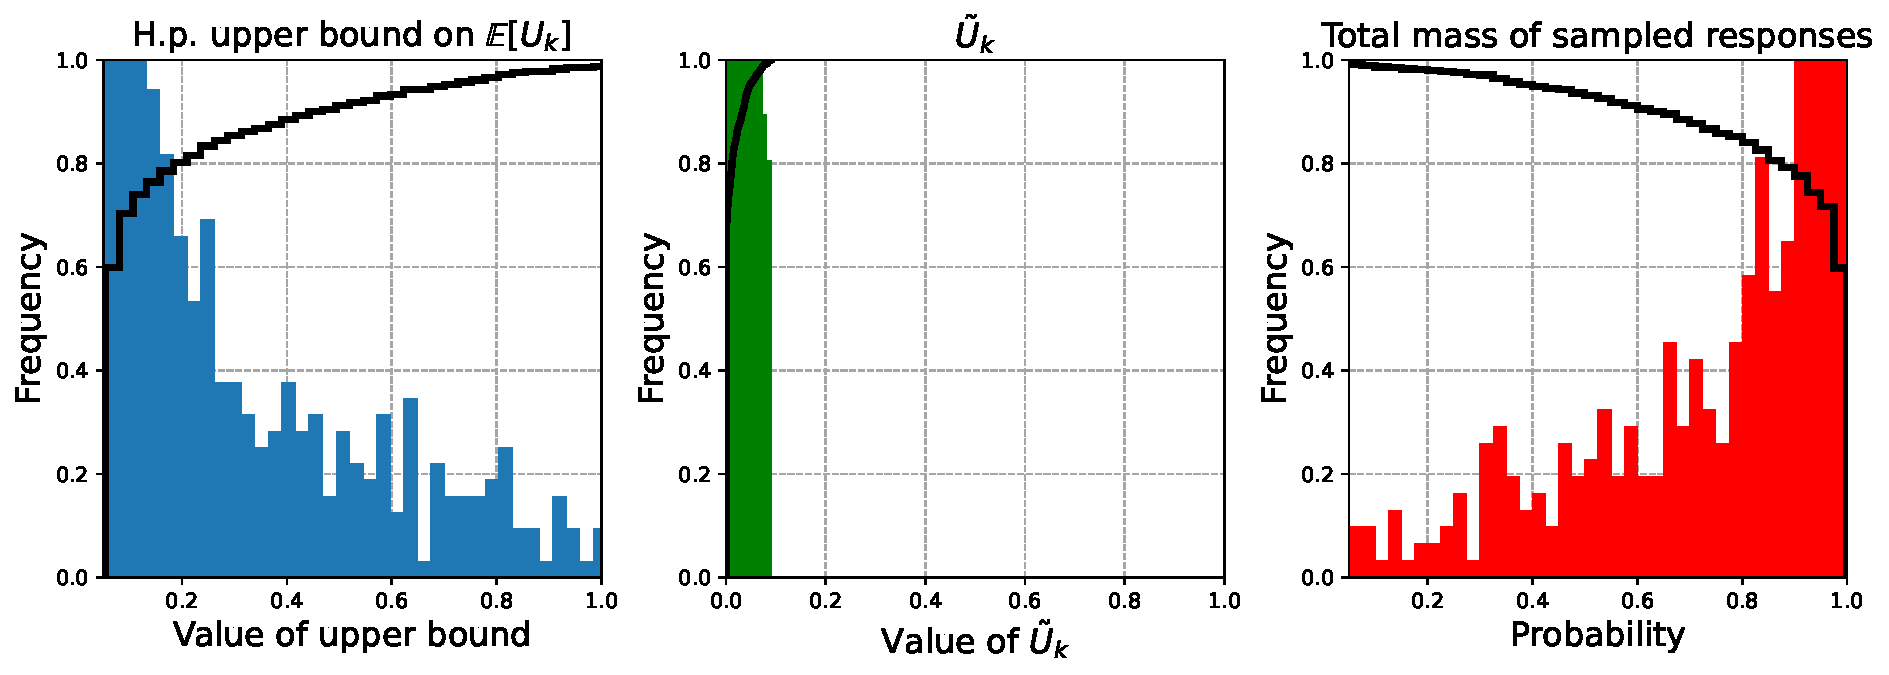
\includegraphics[width=\textwidth]{trivia_qa_missing_mass_with_cdf.pdf}
    \caption*{TriviaQA dataset}
  \end{subfigure}
  \begin{subfigure}[b]{0.48\linewidth}
    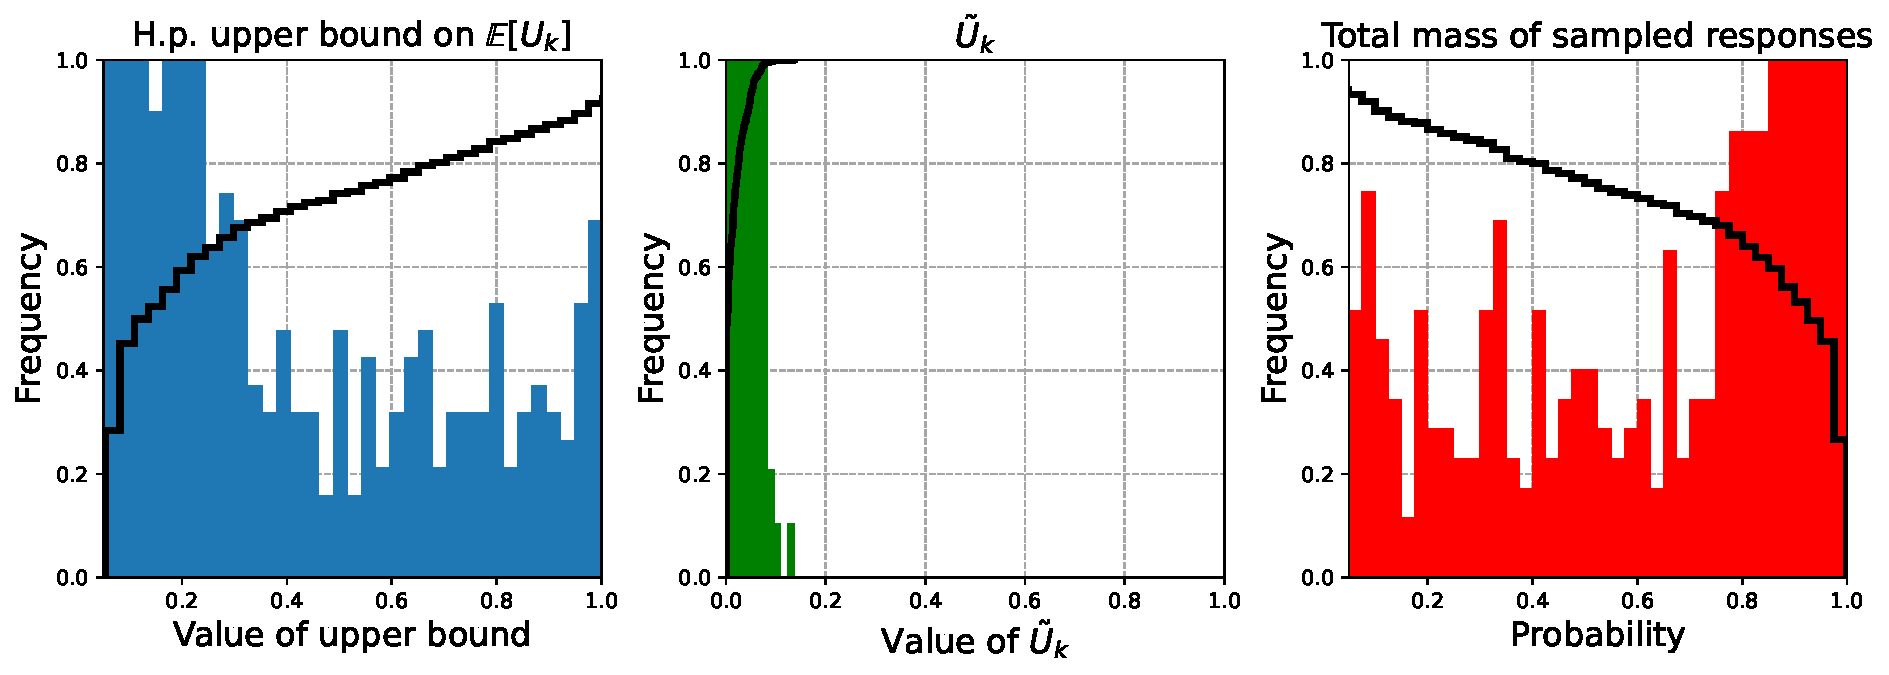
\includegraphics[width=\textwidth]{ambig_qa_missing_mass_with_cdf.pdf}
    \caption*{AmbigQA dataset}
  \end{subfigure}
  \caption{Distributions of bounds on the missing mass. The left figure for each dataset presents the empirical distribution of the upper bounds on the missing mass $\E[U_k]$. %, where each observation is obtained for a separate query.
    The middle figure presents the empirical distribution of $\tilde U_k$, the missing mass computed on a finite support approximation (where the support is obtained by taking samples from the LLM until a cumulative probability of 95\% or 1000 samples are achieved).
    The right graph shows the empirical distribution of $P(\tilde \cX)$, the cumulative probabilities of all responses generated by the language model. For each figure, one observation (sample) corresponds to a single query.
    The black curves represent the corresponding empirical cumulative distribution functions for the upper bounds on $\E{U_k}$ and for $\tilde U_k$, and the empirical survival function (1 minus the empirical distribution function) for the distribution of $P(\tilde \cX)$.
  }
  \label{fig:missing-mass}
\end{figure}
%
%%% Local Variables:
%%% mode: latex
%%% TeX-master: "main_arxiv"
%%% End: